\section{Symptom and Life Event Definition}
\label{sec:appendixA}

We consider a total of 7 mental disorders and 38 symptoms following \citet{Zhang2022SymptomIF}, which are deduced and integrated from DSM-5 \cite{american2013diagnostic}. The 7 disorders and their representative symptoms are listed in the Table \ref{tab:diseases}. And all of the 38 symptoms are listed in the Table \ref{tab:symp_id}. Additionally, we merge the 43 life events in Holmes-Rahe Stress Inventory \cite{Noone2017stress} into 11 classes of life events, as illustrated in Table \ref{tab:all_LEs}. 

\begin{table}[th]
    \small
    \centering
    \begin{tabular}{l|l}
    \hline
    Disease & Typical Symptoms  \\ 
    \hline
    Anxiety  & anxious mood;panic fear \\ \hline
    ADHD  & inattention;hyperactivity;impulsivity	 \\ \hline
    Bipolar Disorder  & drastic shift in mood and energy	  \\ \hline
    Depression & depressed mood;suicidal ideas	   \\ \hline
    Eating Disorder & \makecell[l]{compensatory behaviors to prevent\\ weight gain}	  \\ \hline
    OCD & obsession;compulsions \\ \hline
    PTSD & intrusion symptoms;sleep disturbance \\
    \hline
    \end{tabular}
    \caption{7 Diseases and their Representative Symptoms}
    \label{tab:diseases}
\end{table}

\begin{table}[th]
    \small
    \centering
    \begin{tabular}{l|ccc}
    \hline
    Life events & kappa  \\ 
    \hline
    Loss and Bereavement  & 0.91 \\ 
    Marriage and Commitment  & 0.91	 \\ 
    Relationship Conflicts and Breakdown  & 0.89	  \\ 
    Family Additions and Departures & 0.37	   \\ 
    Health and Well-being & 0.91	  \\ 
    Work and Career Challenges & 0.98 \\ 
    Financial Challenges & 0.89 \\
   
    Education Transitions & 0.92 \\
    
    Change in Living Environment and Habits & 0.82 \\
    
    Vacations and Holidays & 0.92 \\
    
    Legal Matters & 0.93 \\
    \hline
    \textbf{Average} & 0.86 \\
    \hline
    \end{tabular}
    \caption{Agreement (Fleiss' Kappa) of three annotator in the annotation of Life Event Dataset}
    \label{tab:kappa}
\end{table}

\begin{table}[th]
    \small
    \centering
    \begin{tabular}{m{0.4cm}m{6cm}}
    \hline
    id & Symptom  \\
    \hline
    1&Anger Irritability	\\
    2&Anxious Mood 	\\
    3&Autonomic symptoms	\\
    4&Cardiovascular symptoms		\\
    5&Catatonic behavior\\
    6&Decreased energy tiredness fatigue	\\
    7&Depressed Mood\\
    8&Gastrointestinal symptoms	\\
    9&Genitourinary symptoms	\\
    10&Hyperactivity agitation	\\
    11&Impulsivity		\\
    12&Inattention	\\
    13&Indecisiveness	\\
    14&Respiratory symptoms\\
    15&Suicidal ideas	\\
    16&Worthlessness and guilty	\\
    17&Avoidance of stimuli	\\
    18&Compensatory behaviors to prevent weight gain	\\
    19&Compulsions		\\
    20&Diminished emotional expression		\\
    21&Do things easily get painful consequences	\\
    22&Drastic shift in mood and energy	\\
    23&Fear about social situations	\\
    24&Fear of gaining weight	\\
    25&Fears of being negatively evaluated	\\
    26&Flight of ideas	\\
    27&Intrusion symptoms	\\
    28&Loss of interest or motivation	\\
    29&More talkative\\
    30&Obsession	\\
    31&Panic fear	\\
    32&Pessimism	\\
    33&Poor memory	\\
    34&Sleep disturbance	\\
    35&Somatic muscle		\\
    36&Somatic symptoms others		\\
    37&Somatic symptoms sensory	\\
    38&Weight and appetite change	\\
    \hline
    \end{tabular}
    \caption{Id and its corresponding symptoms}
    \label{tab:symp_id}
\end{table}

\begin{table}[th]
    \small
    \centering
    \begin{tabular}{m{0.2cm}m{2.8cm}m{3.5cm}}
    \hline
    id & Life Event Categories & Original Life Events  \\ 
    \hline
    1 & Loss and Bereavement  &    \makecell[l]{Death of a spouse;\\Death of a close family \\member;\\Death of a close friend} \\ \hline
    2 & \makecell[l]{Marriage and \\Commitment}  &  \makecell[l]{Marriage;\\Marital reconciliation}   \\ \hline
    3 & \makecell[l]{Relationship \\ Conflicts \\and Breakdown}  &   \makecell[l]{Divorce;\\Marital separation;\\Change in number of\\ arguments \\with spouse;\\Trouble with in-laws}  \\ \hline
    4 & \makecell[l]{Family Additions and \\Departures}  &  \makecell[l]{Son or daughter leaving\\ home;\\Gain of new family member} \\ \hline
    5 & Health and Well-being  &  \makecell[l]{Personal injury or illness;\\Sex difficulties;\\Pregnancy;\\Change in health of family\\ member} \\ \hline
    6 & \makecell[l]{Work and Career\\ Challenges}  &  \makecell[l]{Fired at work;Retirement;\\Change in responsibilities\\ at work;\\Change to a different line \\of work;\\Spouse begins or stops work;\\Trouble with boss;\\Change in work hours or\\ conditions;\\Business readjustment }\\ \hline
    7 & Financial Challenges &  \makecell[l]{Change in financial state;\\A large mortgage or loan;\\Foreclosure of mortgage or\\ loan;\\A moderate loan or mortgage} \\ \hline
    8 & Education Transitions &  \makecell[l]{Begin or end school/college;\\Change in school/college} \\ \hline
    9 & \makecell[l]{Change in Living\\ Environment and Habits} &  \makecell[l]{Change in living conditions;\\Revision of personal habits;\\Change in sleeping habits;\\Change in eating habits;\\Change in church activities;\\Change in residence;\\Change in recreation;\\Change in social activities;\\Change in number of family \\get-togethers }\\ \hline    
    10 & Vacations and Holidays & \makecell[l]{Vacation;\\Christmas} \\ \hline
    11 & Legal Matters &  \makecell[l]{Jail term;\\Minor violations of the law }\\
    \hline
    \end{tabular}
    \caption{All life events and the 11 major categories}
    \label{tab:all_LEs}
\end{table}

\section{Life Events Dataset}
\label{apd:LE_dataset}
We adopted an annotation similar to that of previous work~\cite{Zhang2022SymptomIF}. Our life event dataset contains 2643 posts related to one or more life events, alongside 5000 control posts (i.e., posts unrelated to any life event). We engaged three experienced annotator for the task, and their agreement (Fleiss' Kappa) is showed in Table\ref{tab:kappa}.


\section{Detailed Symptom and Life Event Identification Results}
\label{sec:symp_ident_res}
The detailed identification results of Symptom and Life Event Identification Models are illustrated in Figure \ref{fig:symptoms_auc_f1} and Figure \ref{fig:LEs_auc_f1} respectively. The high auc and F1 scores show that using these classifiers can help us automatically and accurately extract psychiatric symptoms and life events on Reddit corpus. 
\begin{figure*}[th]
	\centering
	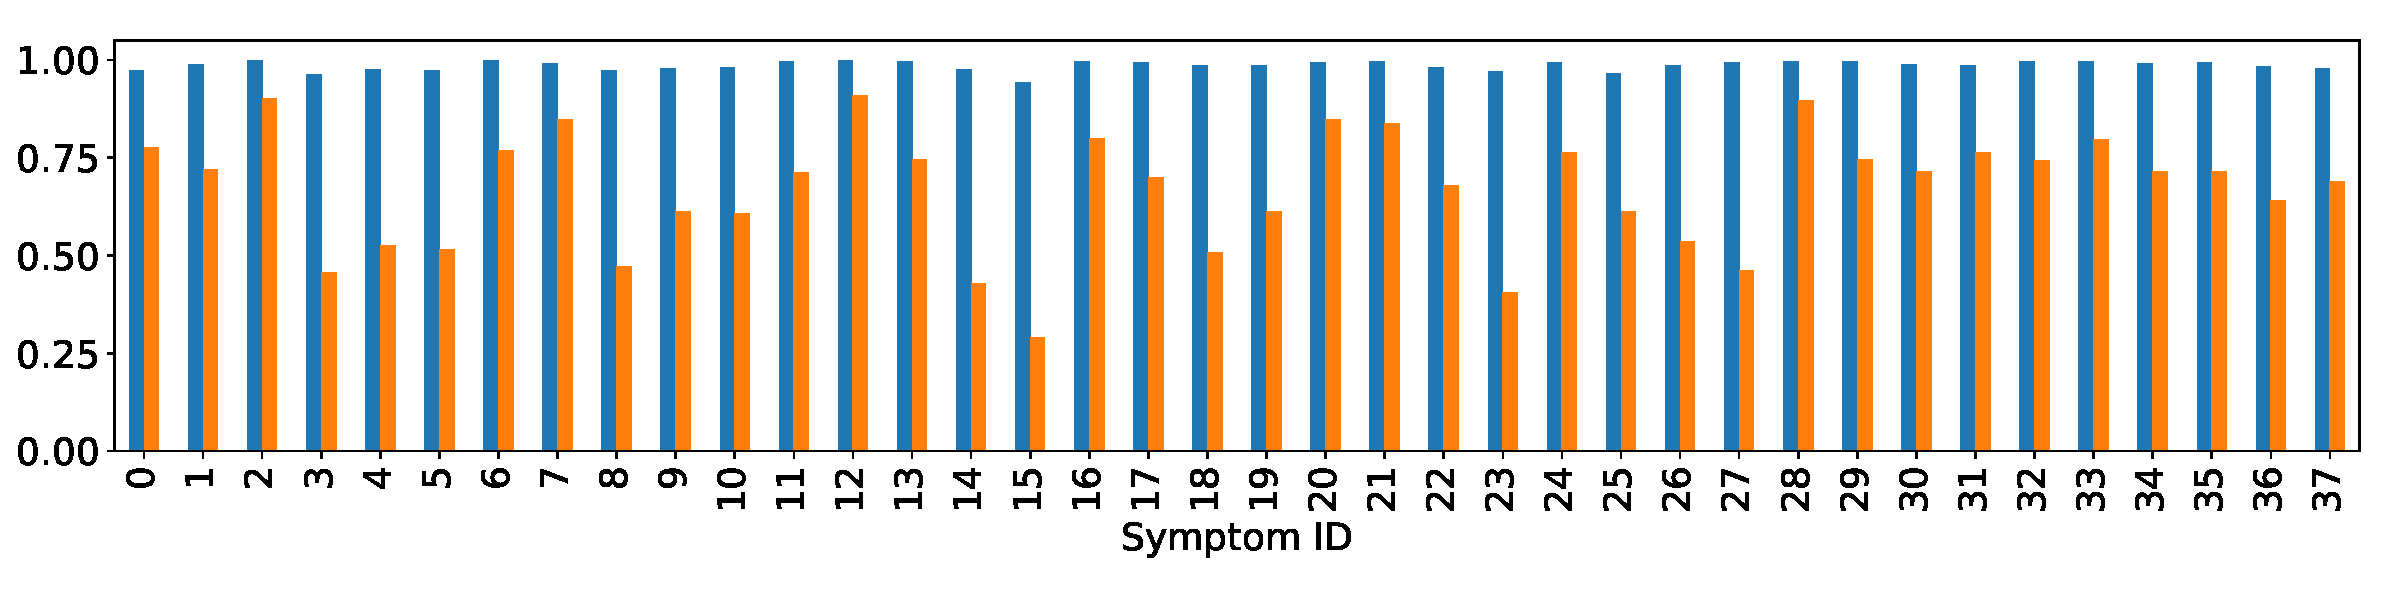
\includegraphics[width=\linewidth]{figures/Symptom_AUC_F1_Multi_disease.pdf}
	\caption{Identification performance of each symptom. The blue bar shows the AUC while the orange bar shows F1, and Symptom ID follows the order of Table \ref{tab:symp_id}. }
	\label{fig:symptoms_auc_f1}
\end{figure*}

\begin{figure*}[th]
	\centering
	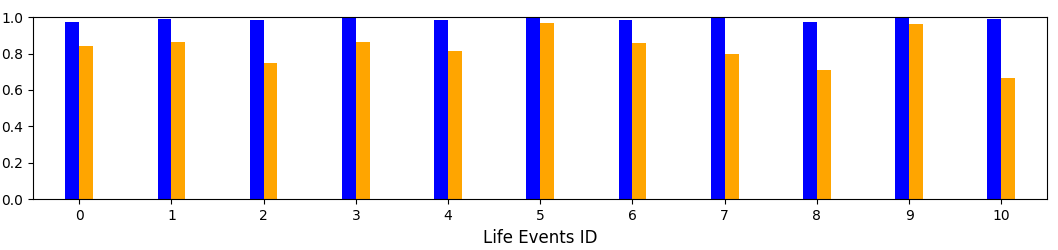
\includegraphics[width=\linewidth]{figures/LEs_auc_f1.png}
	\caption{Identification performance of each life event. The blue bar shows the AUC while the orange bar shows F1, and Life Event ID follows the order of Table \ref{tab:all_LEs}. }
	\label{fig:LEs_auc_f1}
\end{figure*}

% \begin{table}[th]
%     \small
%     \centering
%     \begin{tabular}{m{2.2cm}|m{4cm}}
%         \hline
%         Disease          & Typical Symptoms \\
%         \hline
%         ADHD             & inattention; hyperactivity and impulsivity.         \\
%         \hline
%         Anxiety          &  excessive fear and worry; panic attacks; anxious mood.       \\
%         \hline
%         Bipolar Disorder & drastic shift in mood and energy; experience periods of mania and depression.        \\
%         \hline
%         Depression       &  depressed mood; loss of pleasure or interest; poor concentration; guilty feelings; suicidal ideas.      \\
%         \hline
%         Eating Disorder  &  intense fear of gaining weight; binge and purge; rumination; weight and appetite change.        \\
%         \hline
%         OCD              & obsession; compulsion.         \\
%         \hline
%         PTSD             &  often develops after a shocking, dangerous event; flashbacks; bad dreams.        \\
%         \hline
%     \end{tabular}
%     \caption{7 mental disorders detected in our work with their typical symptoms.}
%     \label{tab:disease_intro}
% \end{table}


\begin{figure}[th]
	\centering
	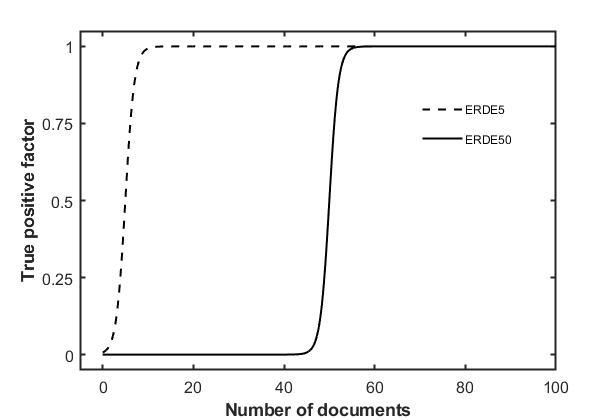
\includegraphics[width=\linewidth]{figures/lco(k).jpg}
	\caption{the cost factor $lc_o(k)$ for $ERDE_5$ and $ERDE_{50}$.}
	\label{fig:lco}
\end{figure}

\section{Causality Results}
\label{sec:appendixB}

\begin{figure*}[th]
	\centering
	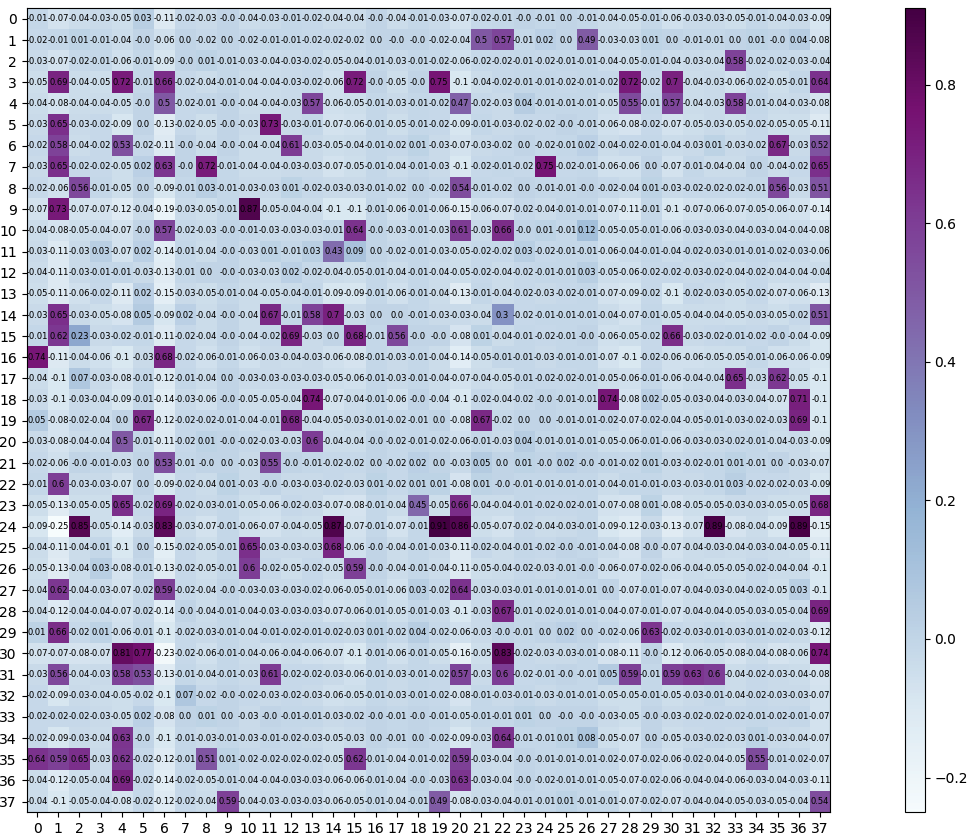
\includegraphics[width=\linewidth]{figures/heat_map_symps_180_2.png}
	\caption{The causal matrix between symptoms with the time window of 180 days. Symptom ID follows the order of Table \ref{tab:symp_id}.}
	\label{fig:heat_map_symps}
\end{figure*}

\begin{figure*}[th]
	\centering
	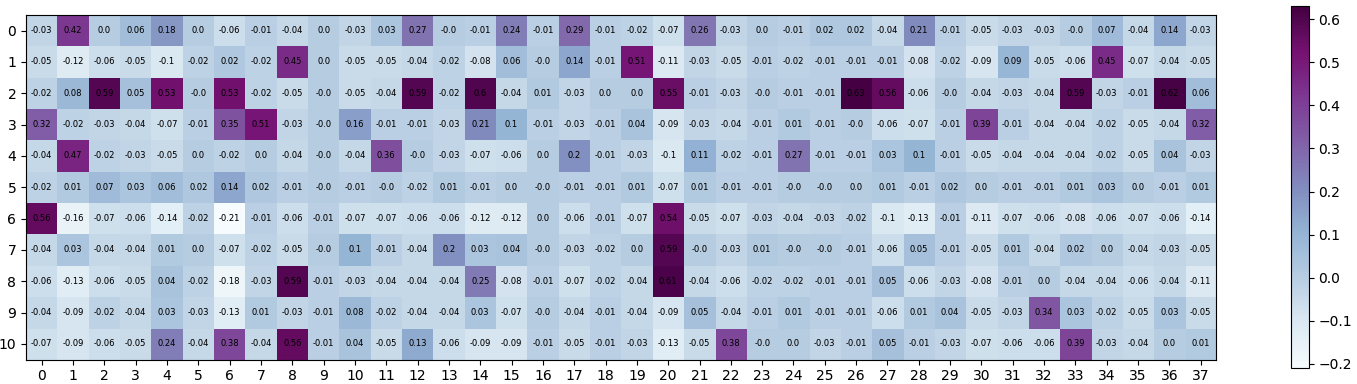
\includegraphics[width=\linewidth]{figures/heat_map_LEs_365_3.png}
	\caption{The causal matrix between LEs and symptoms with the time window of 1 year. Symptom ID and LE ID follow the order of Table \ref{tab:symp_id} and Table \ref{tab:all_LEs}.}
	\label{fig:heat_map_LEs}
\end{figure*}

Here, we present the results of two types of causality in the form of a heatmap. Figure \ref{fig:heat_map_symps} shows the causality between symptoms and Figure \ref{fig:heat_map_LEs} shows the causality between LEs and symptoms. These numbers in figures indicate ATE values of the causal relationships.
% Here, we present the causality between symptoms for time windows of 30 days(Table \ref{tab:syp_causal_30}), 90 days(Table \ref{tab:syp_causal_90}), and 180 days(Table \ref{tab:syp_causal_180}), along with the causality between life events and symptoms. Specifically, for the causality between life events and symptoms, we only showcase the results for a time window of 1 year(Table \ref{tab:LEs_causal_365}). For each time window, we display the top 5 results based on the magnitude of the Average Treatment Effect (ATE) values.



% \begin{table*}[th]
%     \small
%     \centering
%     \begin{tabular}{l|l|cc}
%     \hline
%     Cause Symptom & Result Symptom & ATE & P-value  \\ 
%     \hline
%     fears of being negatively evaluated  & diminished emotional expression	& 0.913	& 0.098 \\
%     fears of being negatively evaluated  & poor memory & 0.894 & 0.061	 \\
%     fears of being negatively evaluated  & somatic symptoms sensory &	0.887 &	0.092	  \\
%     Hyperactivity agitation & Impulsivity & 0.869 & 0.02	   \\
%     panic fear & Decreased energy tiredness fatigue	& 0.767	& 0.06 \\ 
%     \hline
%     \end{tabular}
%     \caption{the causality between symptoms for time window of 180 days}
%     \label{tab:syp_causal_180}
% \end{table*}

% \begin{table*}[th]
%     \small
%     \centering
%     \begin{tabular}{l|l|cc}
%     \hline
%     Cause life Event & Result Symptom & ATE & P-value  \\ 
%     \hline
%     Relationship Conflicts and Breakdown  & intrusion symptoms	& 0.626	& 0.003 \\
%     Relationship Conflicts and Breakdown  & somatic symptoms sensory & 0.618 & 0.082	 \\
%     Relationship Conflicts and Breakdown  & Indecisiveness &	0.593 &	0.091	  \\
%     Change in Living Environment and Habits & Genitourinary symptoms & 0.59 & 0.084	   \\
%     Financial Challenges & Anger Irritability	& 0.565	& 0.079 \\ 
%     \hline
%     \end{tabular}
%     \caption{the causality between life events and symptoms for time window of 1 year}
%     \label{tab:LEs_causal_365}
% \end{table*}

% \begin{table*}[th]
%     \small
%     \centering
%     \begin{tabular}{l|l|cc}
%     \hline
%     Cause Symptom & Result Symptom & ATE & P>|z|  \\ 
%     \hline
%     panic fear  & somatic symptoms sensory	& 0.855	& 0.017 \\
%     avoidance of stimuli  & fears of being negatively evaluated & 0.838 &	0.064	 \\
%     avoidance of stimuli  & sleep disturbance &	0.812 &	0.038	  \\
%     Hyperactivity agitation & panic fear & 0.808 & 0.049	   \\
%     avoidance of stimuli & weight and appetite change	& 0.805	&0.06	  \\ 
%     \hline
%     \end{tabular}
%     \caption{the causality between symptoms for time window of 30 days}
%     \label{tab:syp_causal_30}
% \end{table*}

% \begin{table*}[th]
%     \small
%     \centering
%     \begin{tabular}{l|l|cc}
%     \hline
%     Cause Symptom & Result Symptom & ATE & P>|z|  \\ 
%     \hline
%     fears of being negatively evaluated  & diminished emotional expression	& 0.916	& 0.077 \\
%     fears of being negatively evaluated  & poor memory & 0.875 & 0.065	 \\
%     panic fear  & Decreased energy tiredness fatigue &	0.845 &	0.035	  \\
%     avoidance of stimuli & Inattention & 0.832 & 0.077	   \\
%     panic fear & somatic symptoms others	& 0.83	& 0.099 \\ 
%     \hline
%     \end{tabular}
%     \caption{the causality between symptoms for time window of 90 days}
%     \label{tab:syp_causal_90}
% \end{table*}



\section{Evaluation Metrics}
\label{sec:appendixC}
The following will introduce evaluation metrics for two downstream tasks. $$Precision=\frac{TP}{TP+FP}$$ $$Recall=\frac{TP}{TP+FN}$$
where TP represents true positives (samples correctly predicted as positive),TN represents true negatives (samples correctly predicted as negative), FP represents false positives (samples incorrectly predicted as positive), and FN represents false negatives (samples incorrectly predicted as negative).
Diagnosis Point Detection uses the F1 score as a metric, which balances precision and recall.
$$F1-Score = 2\times\frac{Precision \times Recall}{Precision + Recall}$$

The metric used for early detection of depression, Early Risk Detection Error (ERDE)measure, is defined as follows:

\begin{align*}
\begin{split}
ERDE_o(d,k)= \left \{
\begin{array}{ll}
    c_{fp}    & for \ FP\\
    c_{fn}     & for \ FN\\
    lc_o(k)\cdot c_{tp}    & for\ TP \\
    0     & for\ TN \\ 
\end{array}
\right.
\end{split}
\end{align*}

$c_{fp}$ and $c_{fn}$ are used to adjust the severity of false positives (FP) and false negatives (FN). $c_{fn}$ was set to 1, while $c_{fp}$ is set to the ratio of the number of positive cases in the data to the total number of users. $lc_o(k)$ ($\in [0, 1]$) encodes the cost of delaying the detection of true positives (TP), and $c_{tp}$ defines the level of penalty for delaying TP. Setting $c_{tp}$ to 1  and it means that delaying detection is equivalent to not detecting the case. The function $lc_o(k)$ determines after how many posts k the cost of true positives starts to increase and is defined as follows:
$$lc_o(k)=1-\frac{1}{1+e^{k-o}}$$
The parameter $o$ controls the position on the x-axis where the cost increases more rapidly.We use $ERDE_5$ and $ERDE_{50}$  as evaluation metrics for the results of early detection of depression,shown in Figure \ref{fig:lco}.

\section{Experiment Setting}
\label{sec:appendixD}
In our ERD experiment, we trained the baseline model with the dataset proposed by~\citet{Zhang2022SymptomIF} that originated from a publicly available Reddit corpus. The training process employs a batch size of 64 and learning rate of 0.01. We used symptom features only and the posting list will be limited to a maximum of 256. To prevent over-fitting, we implement early-stopping based on validation performance, with a patience of 4 epochs.



% \section{Statistical significance results}
% \begin{table}[!ht]
%     \small
%     \centering
%     \begin{tabular}{l|c|c}\hline
%     Method  & p-value($ERDE_5$) & p-value($ERDE_{50}$) \\ 
%     \hline
%     baseline vs.{\textit{+symp(30)}} & 0.196 & 0.063   \\ \hline
%     baseline vs.{\textit{+symp(90)}} & 0.024 & 0.331   \\ \hline
%     baseline vs.{\textit{+symp(180)}} & 0.747 & 0.067  \\ \hline
%     baseline vs.{\textit{+symp\&LEs(30)}} & 0.077 & 0.203   \\ \hline
%     baseline vs.{\textit{+symp\&LEs(90)}} & 0.010 & 0.739   \\ \hline
%     baseline vs.{\textit{+symp\&LEs(180)}} & 0.925 & 1 \\ \hline
%     \end{tabular}
% \caption{p-values between the baseline and our method}
%     \label{tab:p-values}
% \end{table}
